% Created 2017-11-22 Wed 16:10
\documentclass[11pt]{article}
\usepackage[utf8]{inputenc}
\usepackage[T1]{fontenc}
\usepackage{fixltx2e}
\usepackage{graphicx}
\usepackage{longtable}
\usepackage{float}
\usepackage{wrapfig}
\usepackage{rotating}
\usepackage[normalem]{ulem}
\usepackage{amsmath}
\usepackage{textcomp}
\usepackage{marvosym}
\usepackage{wasysym}
\usepackage{amssymb}
\usepackage{hyperref}
\tolerance=1000
\author{Tom Shannon}
\date{\today}
\title{valvular\_disease\_notes}
\hypersetup{
  pdfkeywords={},
  pdfsubject={},
  pdfcreator={Emacs 25.3.1 (Org mode 8.2.10)}}
\begin{document}

\maketitle
\tableofcontents

\section{Aortic Stenosis}
\label{sec:AorticStenosis}

\begin{itemize}
\item In descending order of frequency, the three characteristic symptoms of aortic stenosis are
  \begin{itemize}
  \item chest pain (angina pectoris)
    \begin{itemize}
    \item Increased demand, decreased supply (compression)
    \item Sometimes coronary artery disease is present
    \end{itemize}
\item syncope
\item heart failure
\end{itemize}
\item On auscultation, a midsystolic murmur is heard, loudest at the base of the heart, and often with radiation to the sternal notch and the neck.
\item Normal = 3.5 - 4.0 cm$^2$, critical at 0.8 cm$^2$
\item Wall thickens symetcially in an effort to reduce wall stress with very high pressure but cavitary readius remains unchanged - \textbf{concentric hypertrophy}
\item Pressure-volume loop in aortic stenosis.

\begin{itemize}
\item  The left ventricle becomes thickened and less compliant, forcing the diastolic pressure-volume curve upward, which results in elevated left ventricular end-diastolic pressure. 
\item increased afterload
\item hypertrophy of the ventricle results in increased inotropic force
    \end{itemize}
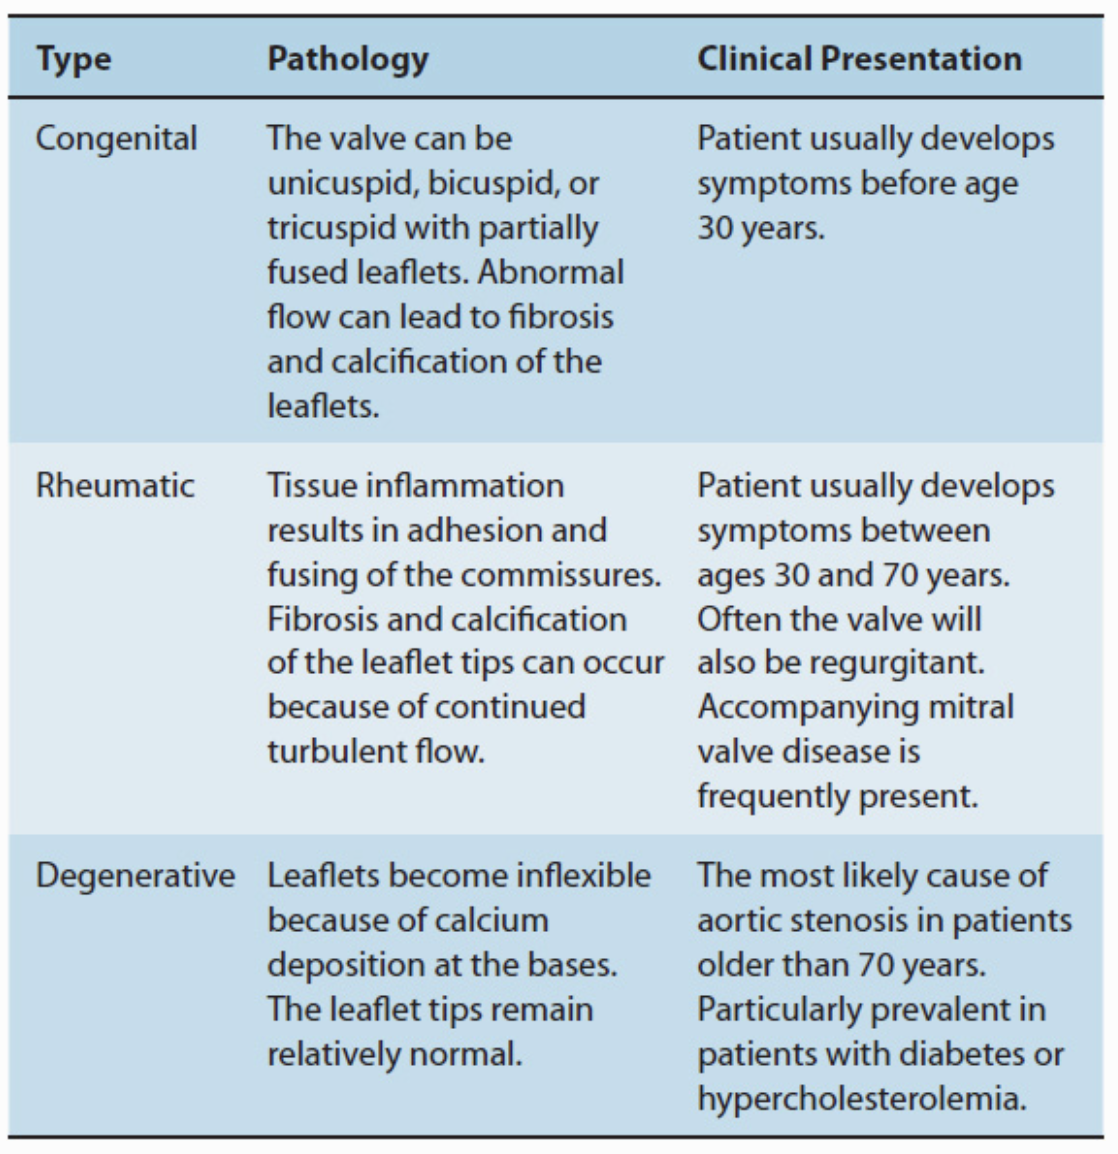
\includegraphics[width=0.45\textwidth]{images/causes_of_aortic_stenosis.png}
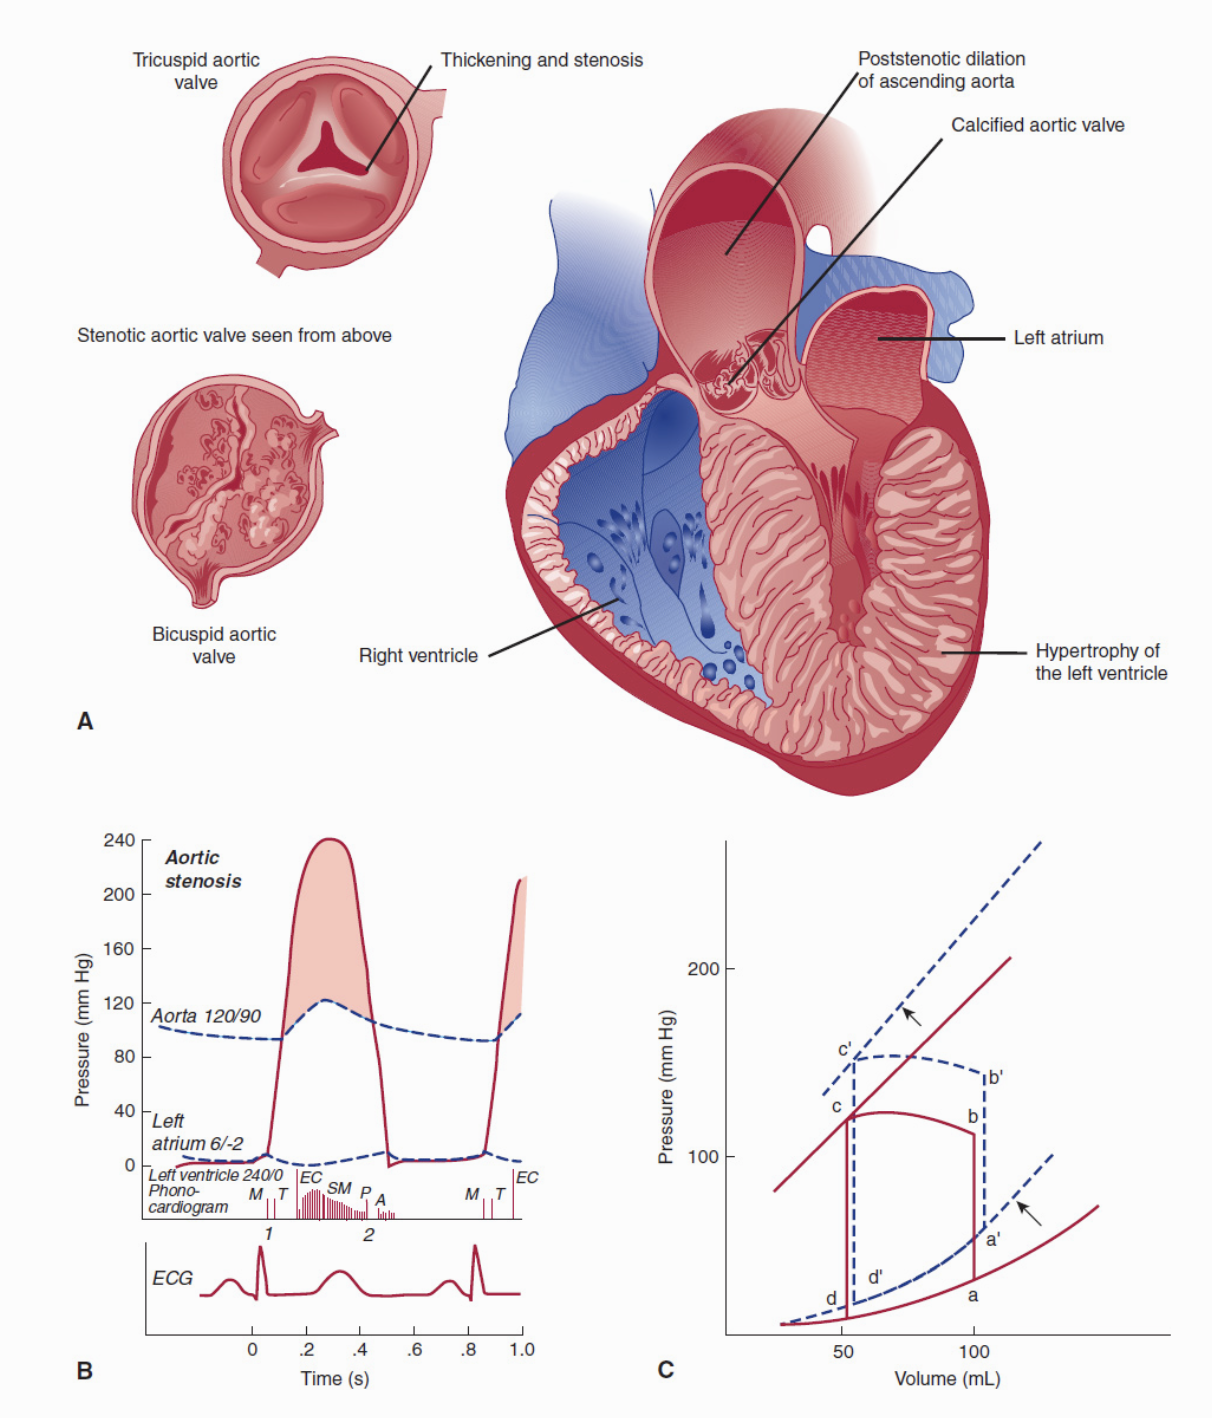
\includegraphics[width=0.45\textwidth]{images/characteristics_of_aortic_stenosis.png}
\end{itemize}

\section{Aortic Regurgitation}
\label{sec:AorticRegurgitation}
\begin{itemize}
\item pounding pulse
\item three murmurs may be heard:
  \begin{itemize}
  \item a high-pitched early diastolic murmur
  \item a diastolic rumble called the Austin Flint murmur - The Austin Flint murmur is thought to result from regurgitant flow from the aortic valve impinging on the anterior leaflet of the mitral valve, producing functional mitral stenosis.
  \item a systolic murmur.
  \end{itemize}

\item Volume overload $\rightarrow$ \textbf{eccentric hypertrophy} where dilation and thickening takes place - the ventricular cavity enlarges laterally in the chest and becomes eccentric to its normal position
\item Pressure-volume loop in chronic aortic insufficiency.
  \begin{itemize}
  \item Marked enlargement in left ventricular volume shifts the
    diastolic pressure-volume curve rightward. 
  \item Hypertrophy of the
    ventricle shifts the isovolumic pressure-volume curve leftward
    (not shown), but ultimately the ventricle dilates and
    contractility decreases and the isovolemic pressure-volume curve
    shifts to the right. 
  \item Stroke volume is enormous
  \item no isovolumic periods exist.
\end{itemize}

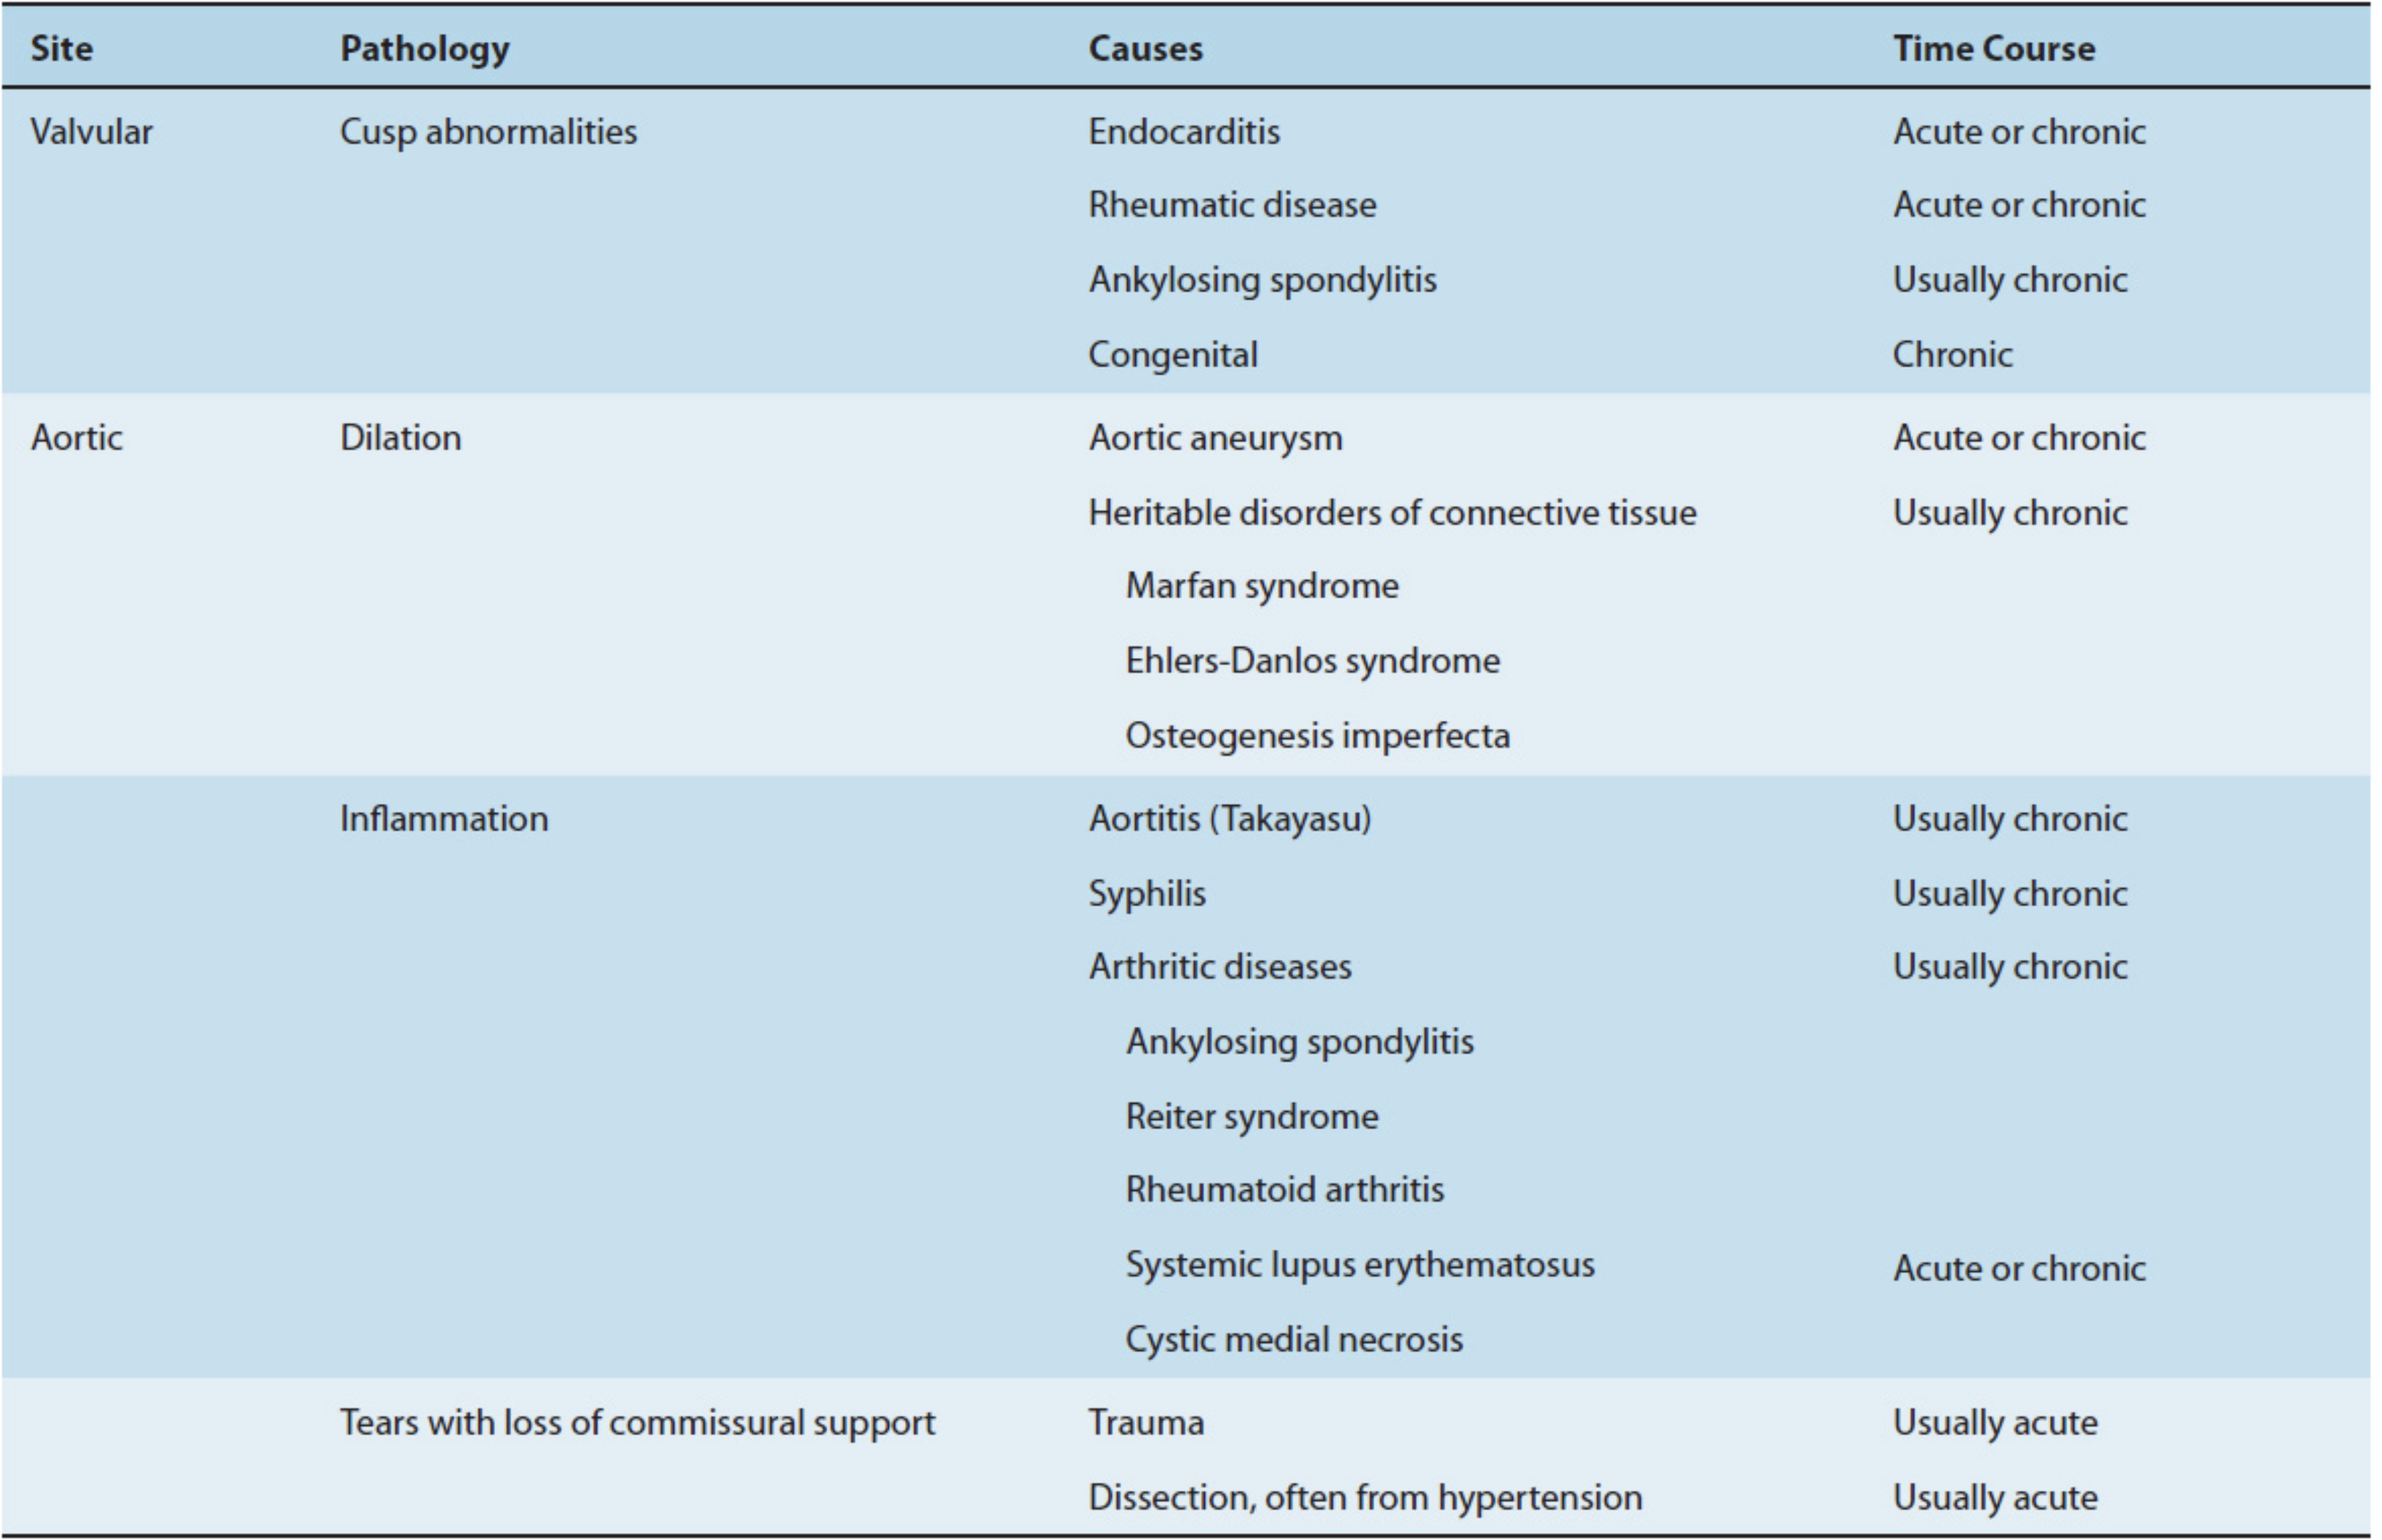
\includegraphics[width=0.45\textwidth]{images/causes_of_aortic_insufficiency.png}
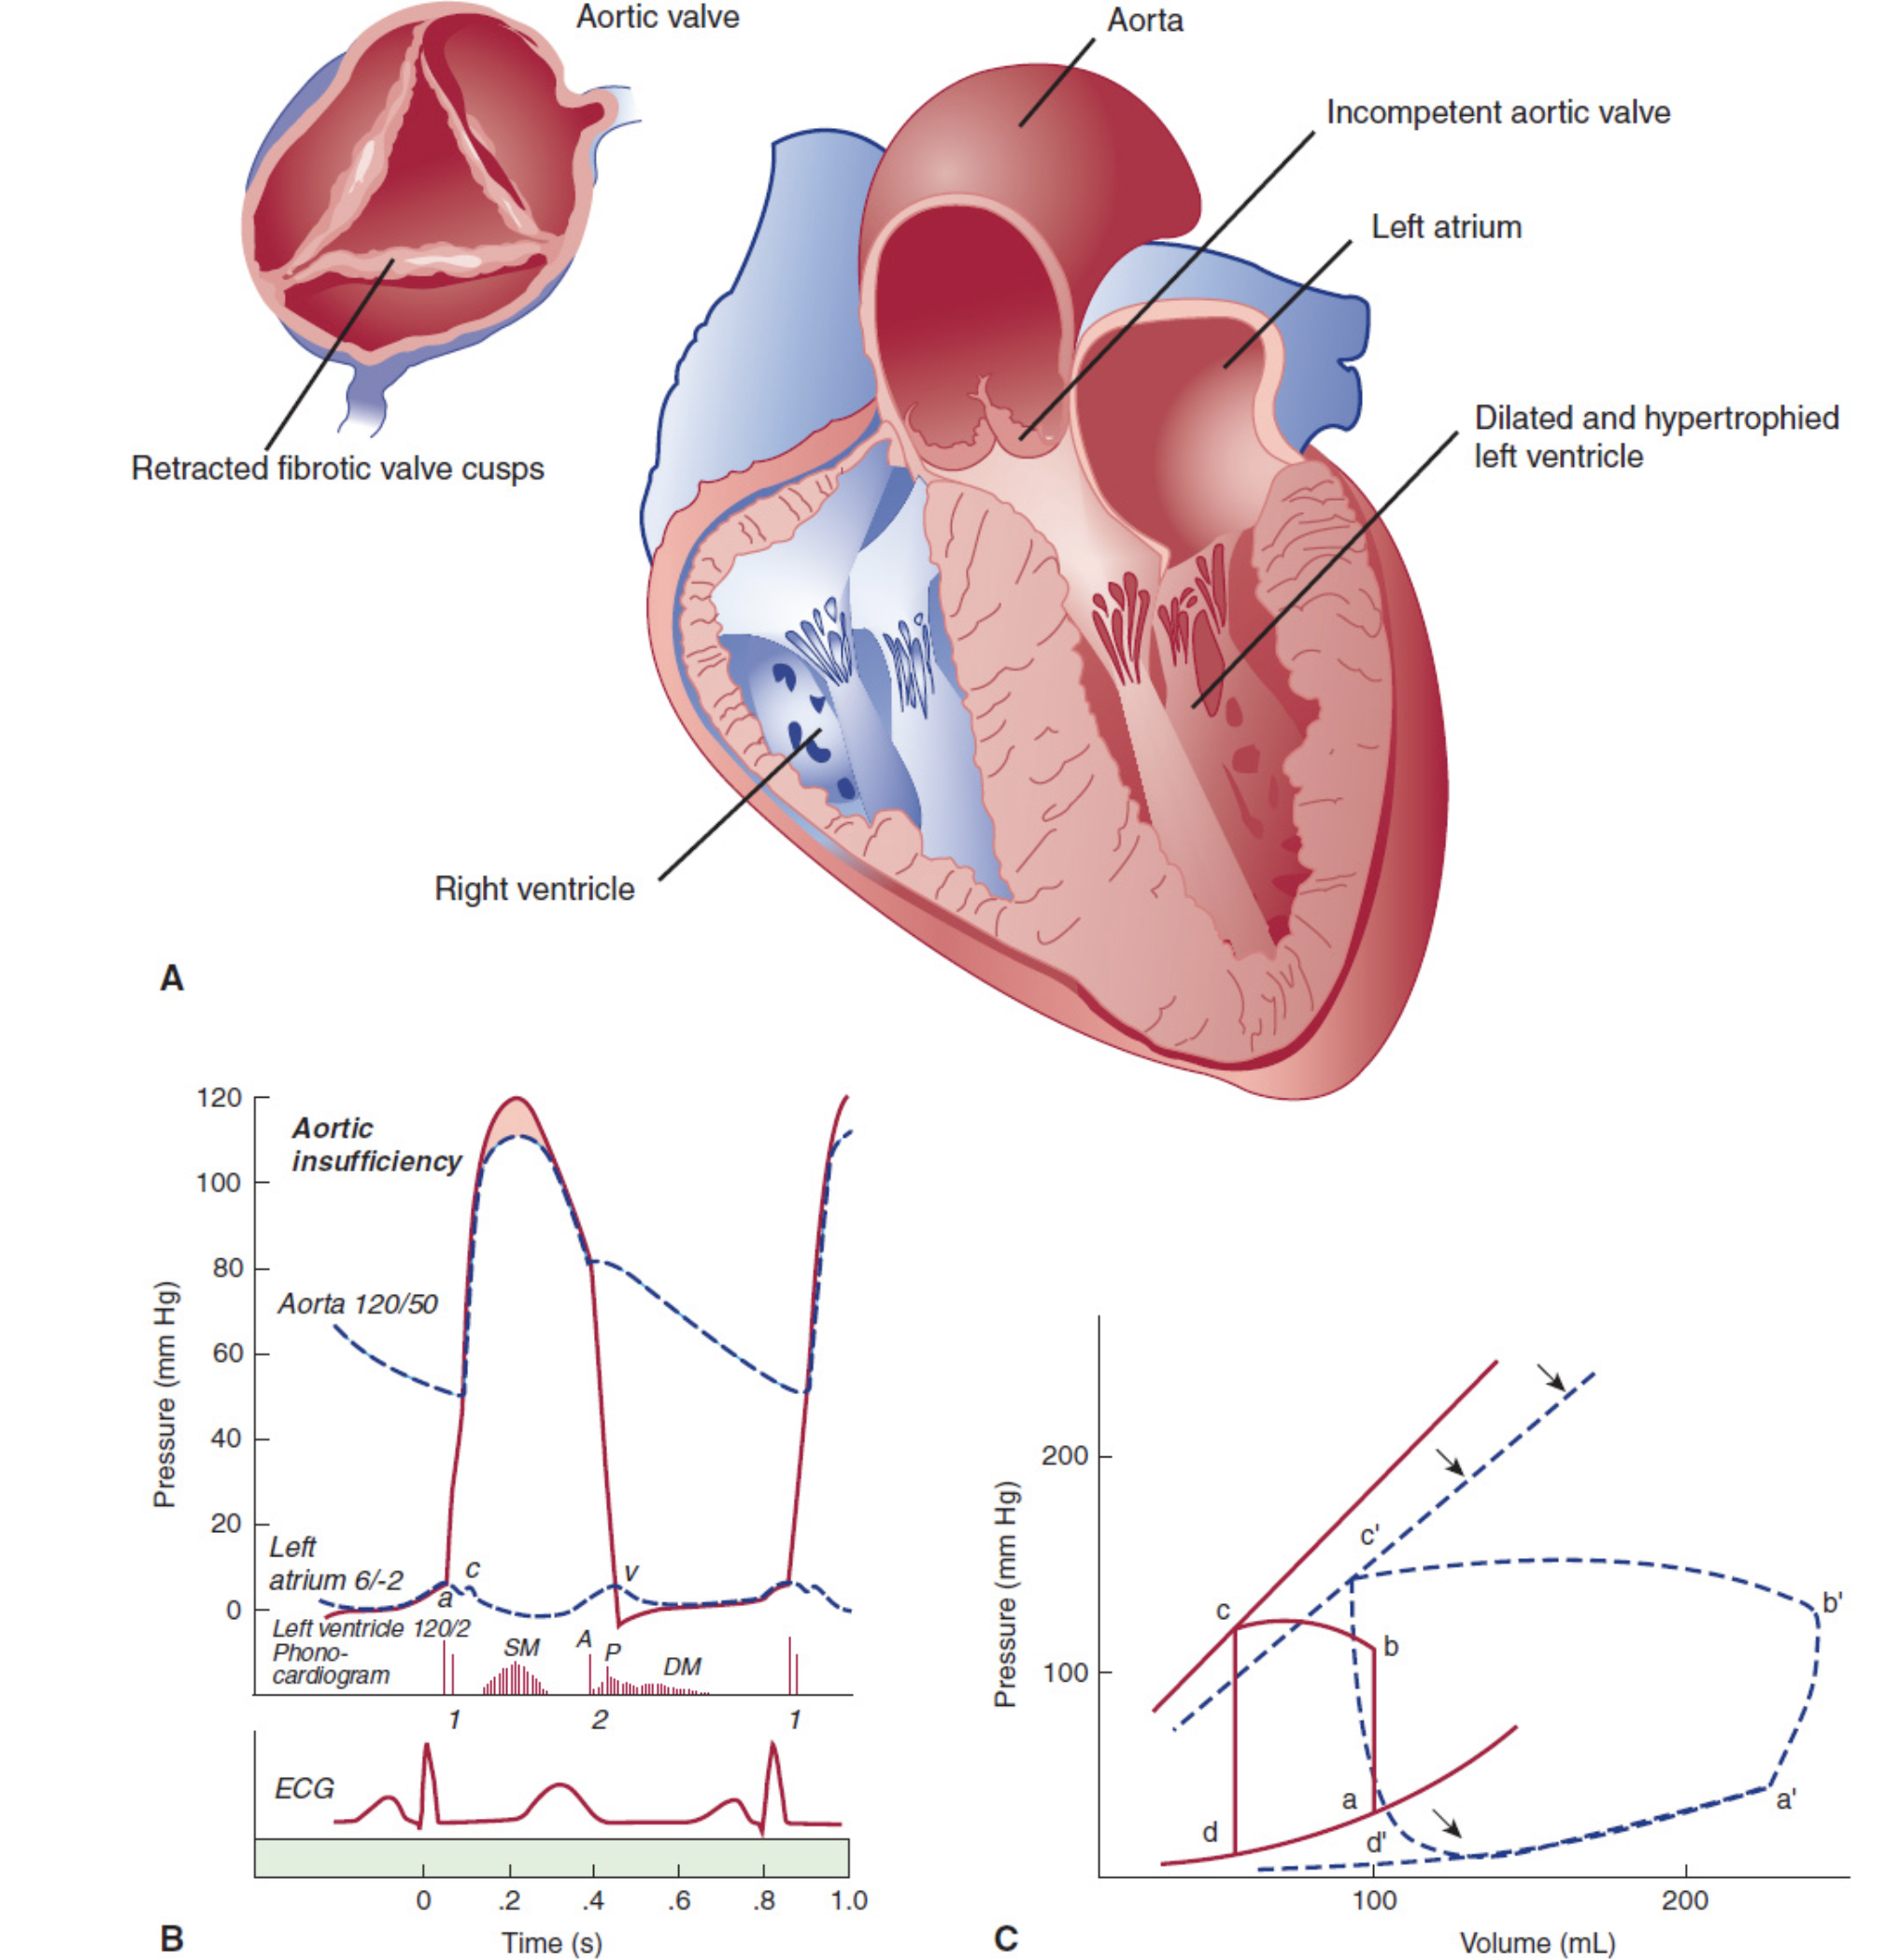
\includegraphics[width=0.45\textwidth]{images/characteristics_of_aortic_insufficiency.png}
\end{itemize}

\section{Mitral Stenosis}
\label{sec:MitralStenosis}

\begin{itemize}
\item The characteristic murmur of mitral stenosis is a late low-pitched diastolic rumble. In addition, an opening snap may be heard in the first portion of diastole.
\item The mitral valve area is usually 5–6 cm2; clinically relevant mitral stenosis usually occurs when the valve area decreases to less than 1 cm2.
\item Atrial enlargement is characteristic and patients are prone to arrhythmias.
\item Reduced outflow leads to dilation of the left atrium and stasis of blood flow. Thrombus in the left atrium is observed on echocardiography in approximately 20\% of patients with mitral stenosis, and the prevalence increases with age, presence of atrial fibrillation, severity of stenosis, and any reduction in cardiac output. Embolic events that lead to neurologic symptoms occur in 8\% of patients in sinus rhythm and in 32\% of patients with chronic or paroxysmal atrial fibrillation. In addition, left atrial enlargement can sometimes impinge on the recurrent laryngeal nerve and lead to hoarseness (Ortner syndrome).
  
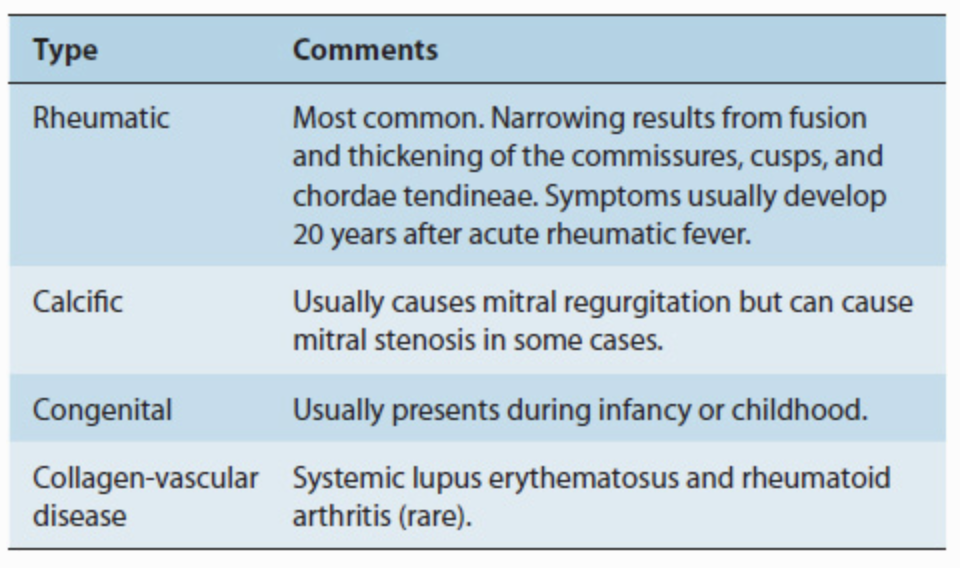
\includegraphics[width=0.45\textwidth]{images/causes_of_mitral_stenosis.png}
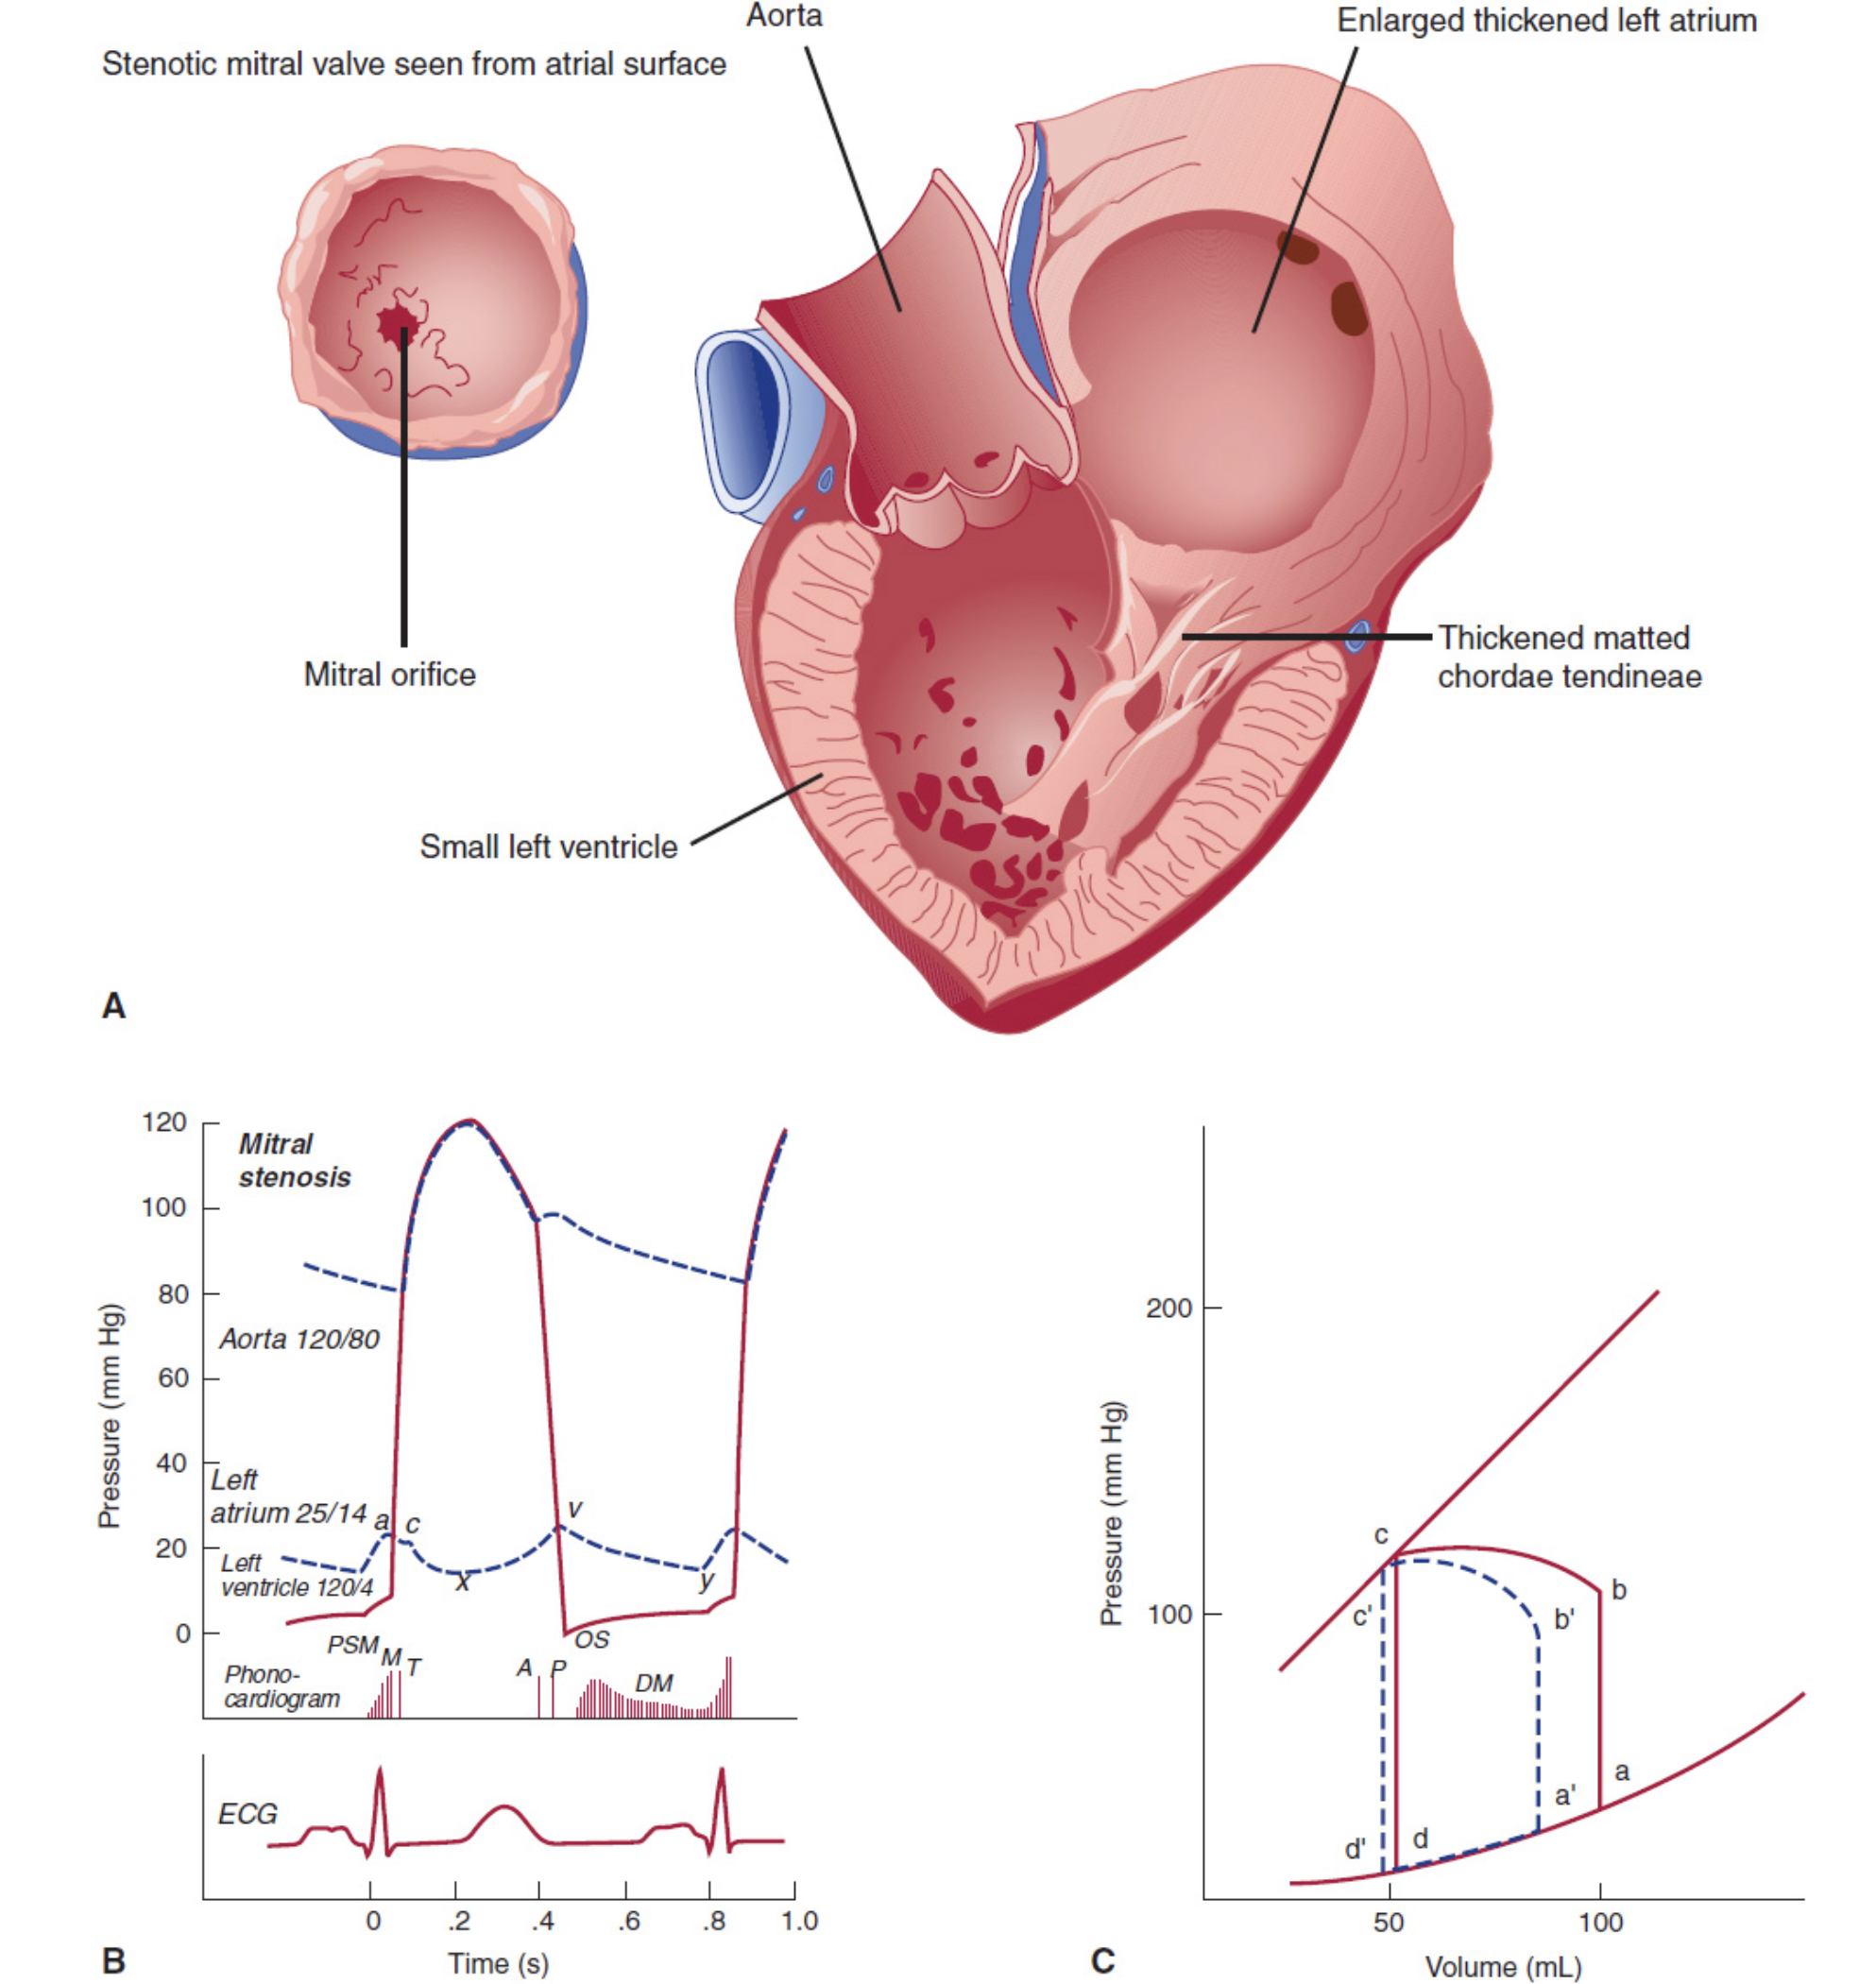
\includegraphics[width=0.45\textwidth]{images/characteristics_of_mitral_stenosis.png}
\end{itemize}

\section{Mitral Stenosis}
\label{sec:MitralStenosis}
\begin{itemize}
\item In the past, rheumatic heart disease accounted for most cases of mitral regurgitation. Mitral valve prolapse is now probably the most common cause, followed by coronary artery disease.
\item Cardinal features include
  \begin{itemize}
  \item left atrial enlargement
    
  \item left ventricular enlargement (hypertrophy in acute lesions)
  \item prominent v wave caused by filling from both the pulmonary veins
    and the regurgitant jet
  \item holosystolic murmur - it is usually heard best at the apex and often radiates to the axilla.
\end{itemize}

\item Pressure-volume loop in mitral insufficiency
  \begin{itemize}
  \item Increased ventricular volumes shift the diastolic
    pressure-volume curve rightward
  \item Stroke volume is increased
  \item isovolemic pressure-volume curve eventually shifts to the right with chronic volume overloads
\end{itemize}

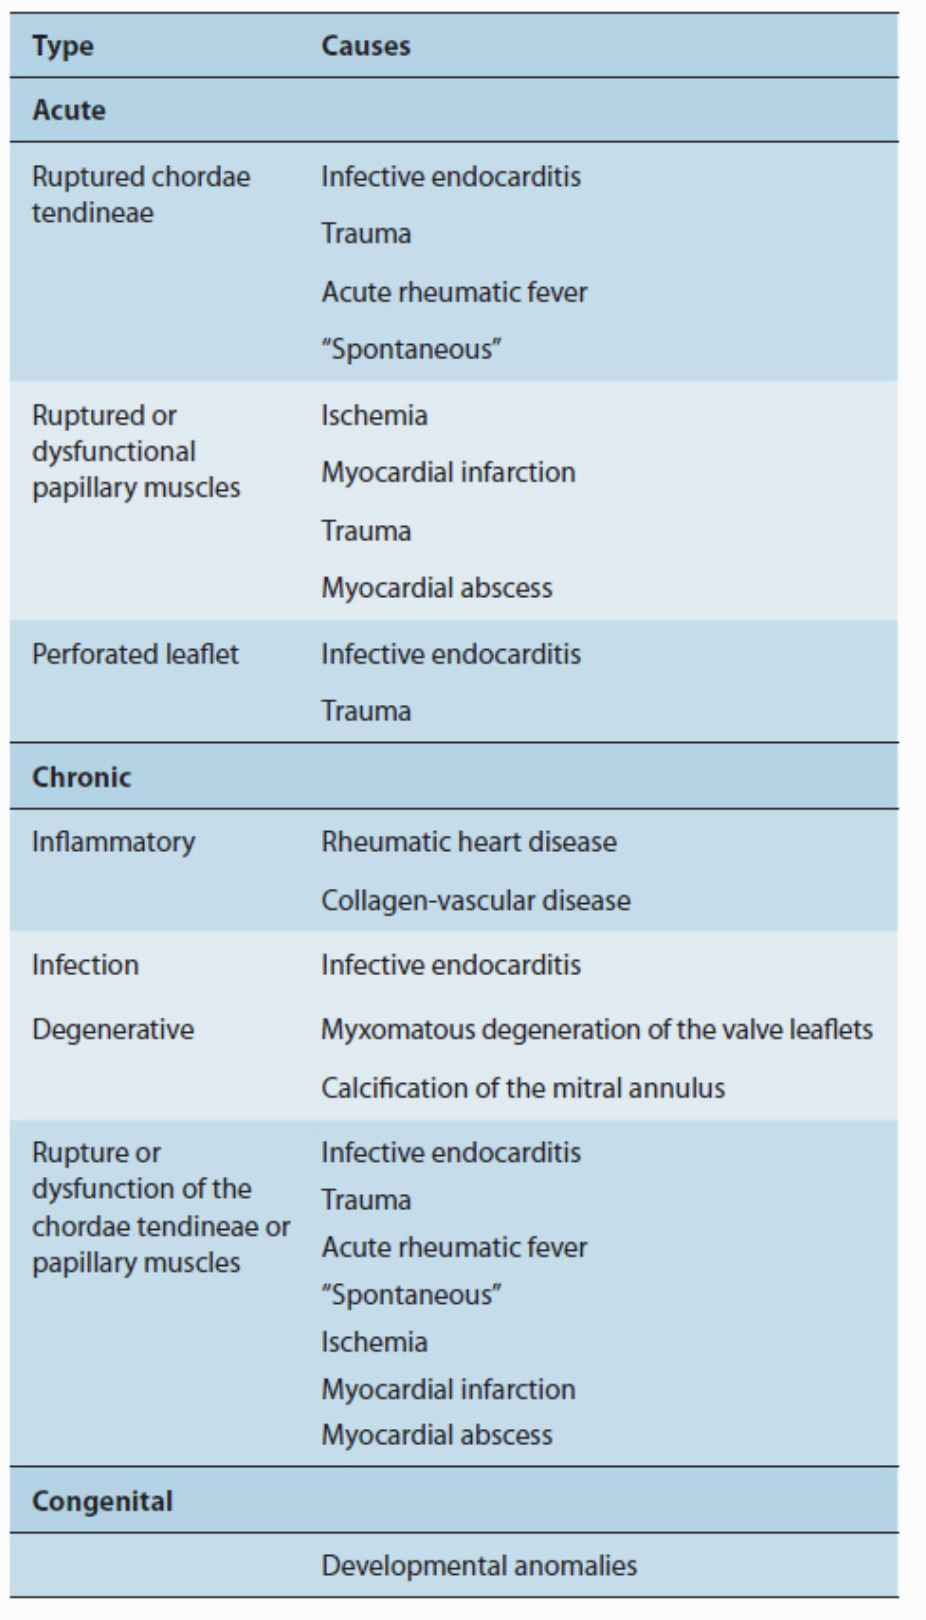
\includegraphics[width=0.45\textwidth]{images/causes_of_mitral_insufficiency.png}
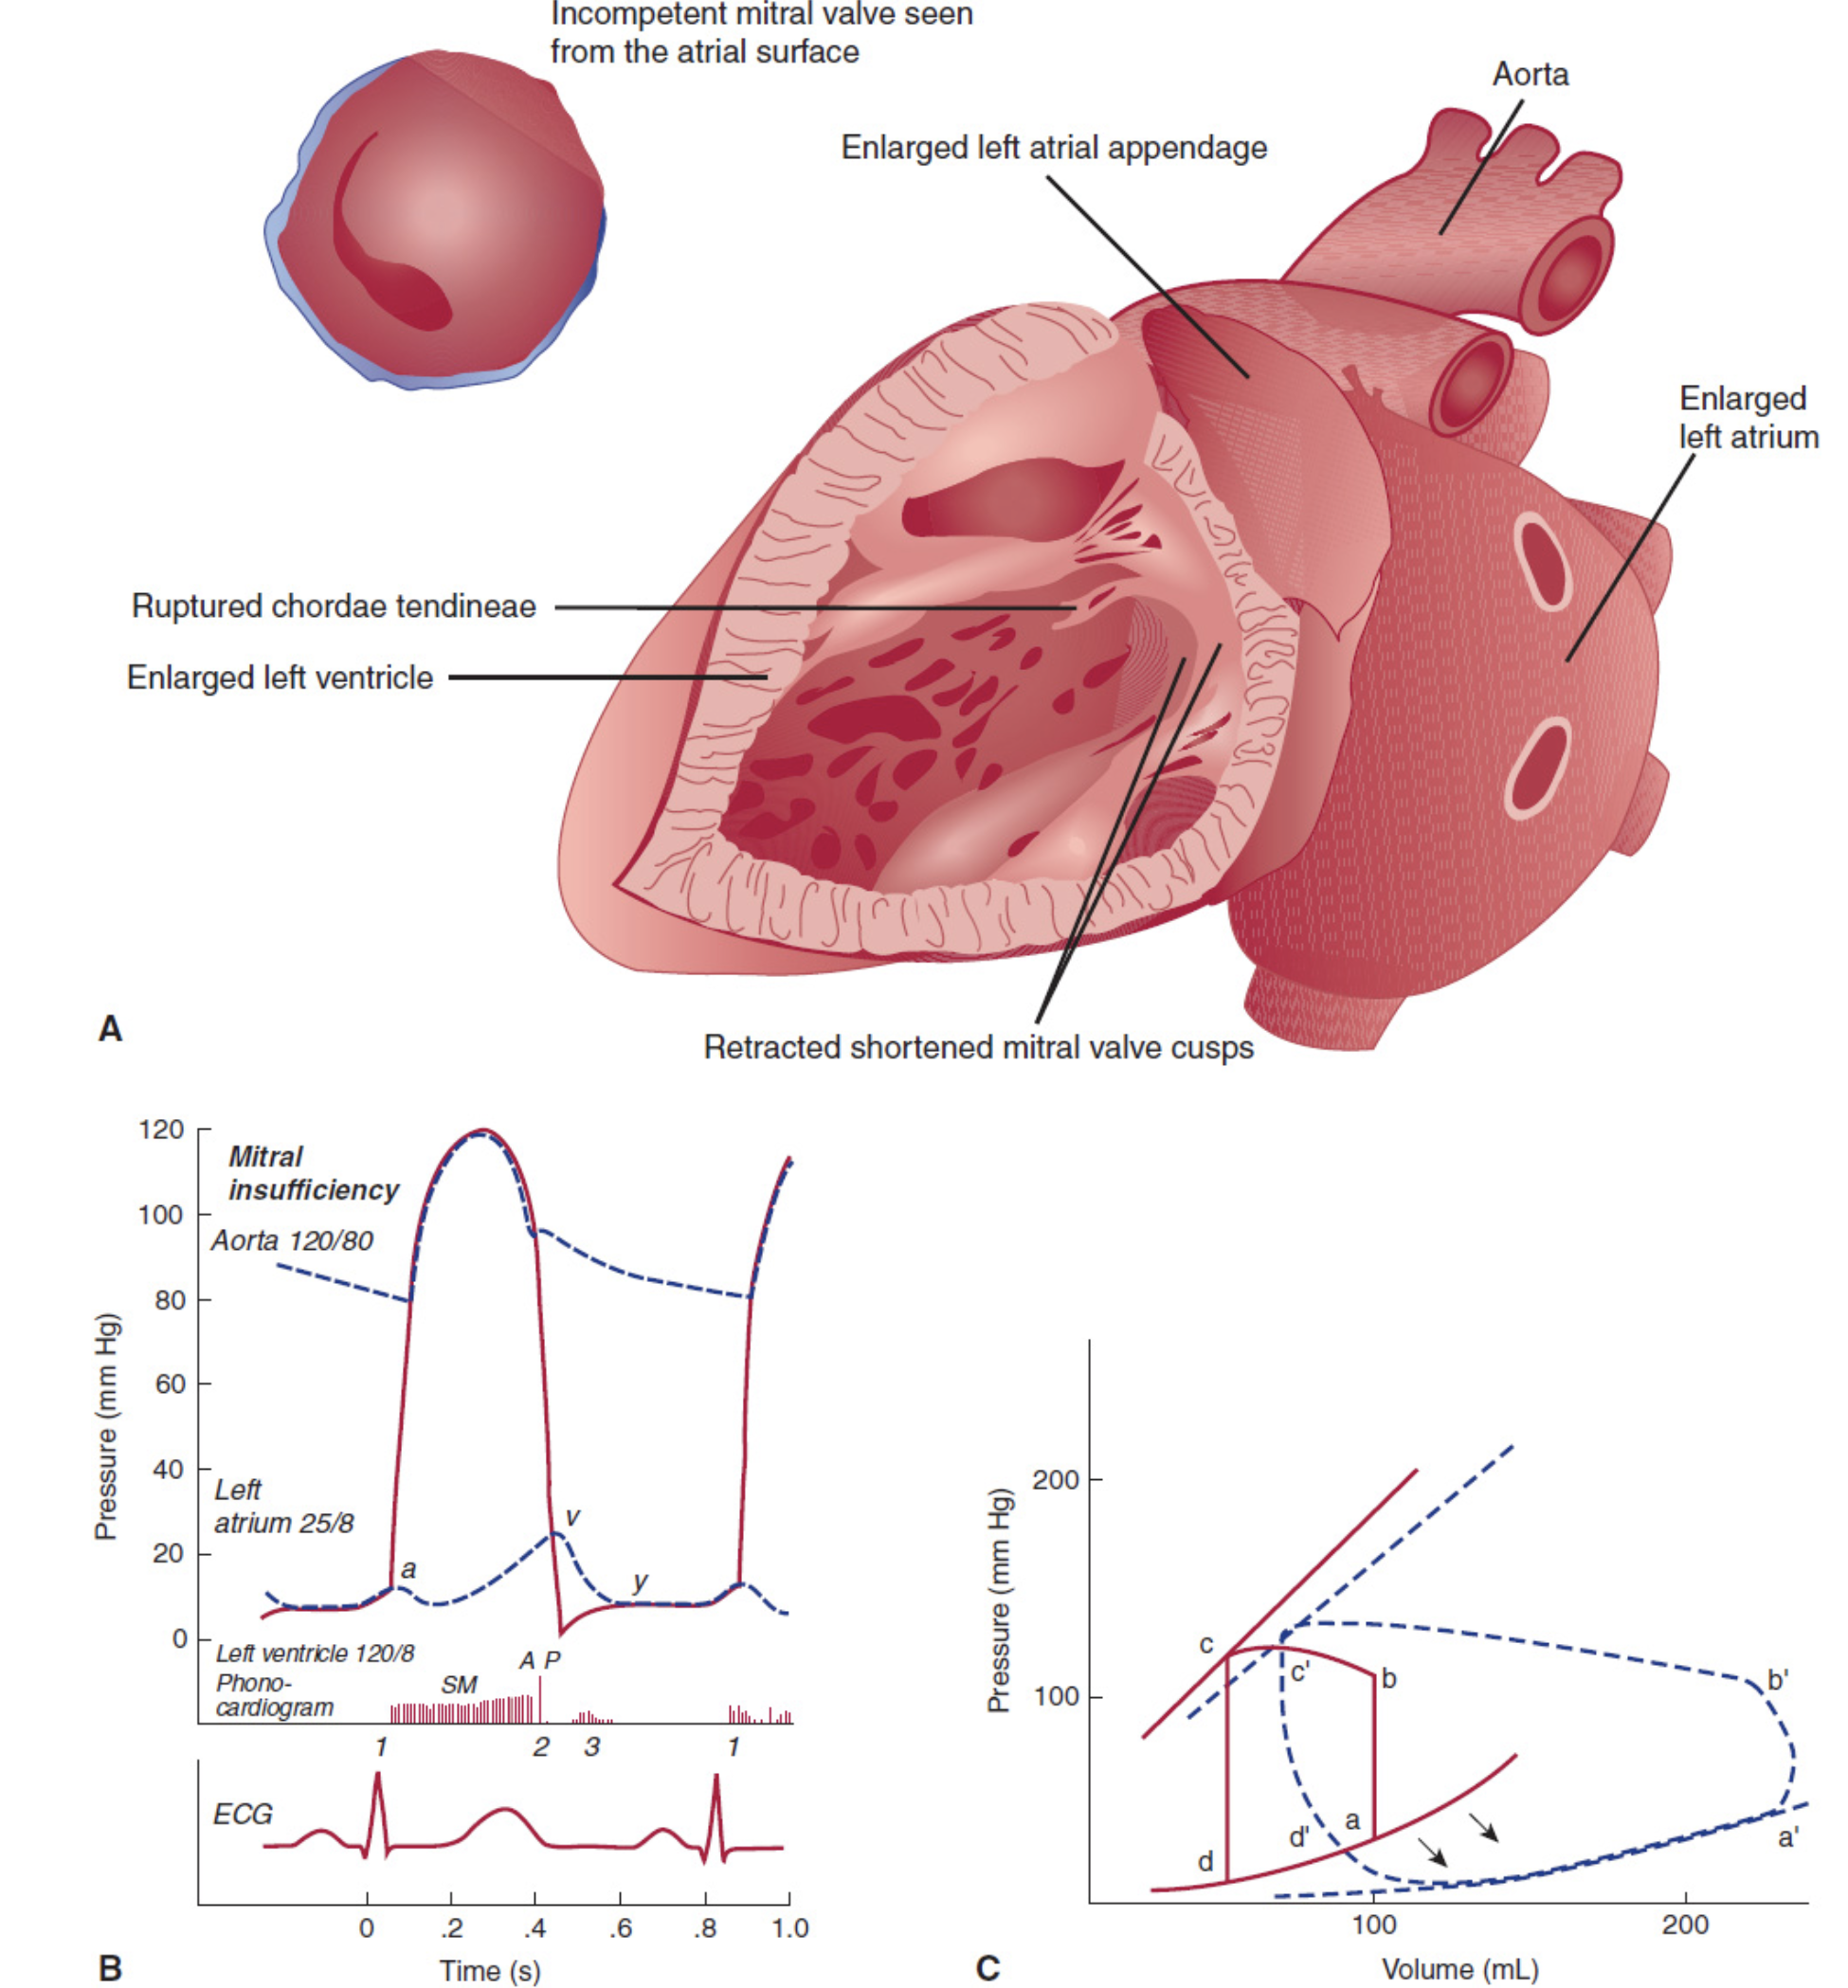
\includegraphics[width=0.45\textwidth]{images/characteristics_of_mitral_insufficiency.png}

\end{itemize}
% Emacs 25.3.1 (Org mode 8.2.10)
\end{document}